\section{Crock Pot Shredded Venison}\index{meat!venison!crock pot shredded}

\begin{center}
Prep Time: 10 min
Total Time: 310 min

\noindent Yield: 16

\vspace{1em}

Source: https://www.food.com/recipe/crock-pot-shredded-venison-sandwiches-84865
\end{center}

\subsection{Ingredients}
\begin{multicols}{2}
\begin{itemize}
    \item 4 lbs boneless venison roast
    \item 1 $\frac{1}{2}$ cups ketchup
    \item 3 tablespoons brown sugar
    \item 1 tablespoon ground mustard
    \item 1 tablespoon lemon juice
    \item 2 tablespoons soy sauce
    \item 1 tablespoon liquid smoke (optional)
    \item 2 teaspoons celery salt
    \item 2 teaspoons Worcestershire sauce
    \item 1 teaspoon onion powder
    \item 1 teaspoon garlic powder
    \item $\frac{1}{8}$ teaspoon ground nutmeg
    \item 3 drops hot pepper sauce, to taste
    \item 14 -18 hamburger buns, split
\end{itemize}
\end{multicols}

\subsection{Preparation}
\begin{enumerate}
    \item Cut venison roast in half; place in a 5 quart. slow cooker.
    \item In a large bowl, combine the ketchup, brown sugar, mustard, lemon juice, soy sauce, liquid smoke if desired and seasonings.
    \item Pour over venison.
    \item Cover and cook on high for 4 1/2 to 5 hours or until meat is tender.
    \item Remove the roast; set aside to cool.
    \item Strain sauce and return to slow cooker.
    \item Shred meat, using two forks; stir into sauce and heat through.
    \item Using a slotted spoon, spoon meat mixture onto each bun.
\end{enumerate}

\begin{figure}[h!]
    \centering
    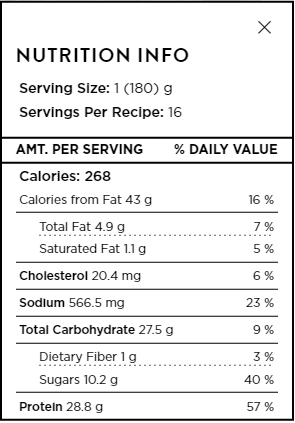
\includegraphics[width=.25\textwidth]{img/crock-pot-shredded-venison-nutrition.png}
    \caption{Nutrition information for crock pot shredded venison.}
    \label{fig:crock-pot-shredded-venison}
\end{figure}